\chapter*{Desarrollo del proyecto}
\addcontentsline{toc}{chapter}{Desarrollo del proyecto}

\section*{Título del proyecto}
\addcontentsline{toc}{section}{Título del proyecto}

Guardabosques Universitarios de la Universidad Simón Bolívar

\section*{Objectivo general}
\addcontentsline{toc}{section}{Objectivo general}

Proveer experiencias centradas en la cultura del árbol y de la apreciación de la biodiversidad, que sensibilicen y hagan participar a los ciudadanos urbanos y peri-urbanos en el mejoramiento de su ambiente.

\section*{Objectivos específicos}
\addcontentsline{toc}{section}{Objectivos específicos}

\begin{itemize}

\item Difundir los valores de la biodiversidad de Caracas.

\item Propagar especies para la arborización y reforestación, y difundir sus técnicas.

\item Arborizar, reforestar y restaurar ambientes degradados.

\item Proteger árboles en el contexto urbano y de los espacios que los contienen.

\item Aplicar las técnicas de los juegos ecológicos ``ecorutas'' para la comunidad.

\end{itemize}

\section*{Actividades realizadas}
\addcontentsline{toc}{section}{Actividades realizadas}

En esta sección se describirán las actividades que fueron realizadas por mi persona durante el trabajo comunitario realizado con los guardabosques universitarios de la Universidad Simón Bolívar. Las mismas se pueden agrupar como se muestran a continuación.

\subsection*{Sociedad Amigos del Árbol}
\addcontentsline{toc}{subsection}{Sociedad Amigos del Árbol}

\begin{itemize}

\item \textbf{Limpieza y barrido de hojas (sede La Floresta):} consistió en barrer las hojas que se desprenden de los árboles que cubren el vivero. También se reorganizó y se limpió la la oficina administrativa que se encuentra dentro de la sede. Estas son actividades rutinarias que se deben realizar periódicamente para mantener un ambiente propicio de trabajo. Estas hojas luego se utilizarán como abono.

\item \textbf{Acondicionamiento de la sede (La Castellana):} la Sociedad Amigos del Árbol dispone de una sede en La Castellana que se encontraba en desuso. Con el fin de proporcionarle utilidad a la misma, se desarrollaron actividades de acondicionamiento. Entre ellas se encuentran el vaciado, barrido y coleteo de los depósitos y la oficina. Esta actividad se realizó una vez. Ahora la Sociedad Amigos del Árbol dispone de dos sedes acondicionadas para prestar un servicio con un mayor alcance a la comunidad.

\item \textbf{Reciclaje de papel:} la sede de la Castellana antes de ser acondicionada se utilizaba como depósito de revistas y periódicos. Algunos de estos periódicos y revistas se encontraban humedecidos por la filtración de agua de lluvia en la sede. Por esta razón se fueron clasificados y el papel que se encontraba en buenas condiciones fue apartado para reciclaje. 

\item \textbf{Actividades de compost:} Consistía en mantener la materia orgánica en el compostero. Al descomponerse la materia, se utiliza como abono para actividades de siembra y trasplante. Esta materia organica se obtiene del barrido de las hojas y del desmalezamiento de las plantas que se encuentran en el vivero de la Sociedad Amigos del Árbol. Es una actividad que se realiza periodicamente.

\item \textbf{Clasificación, limpieza y secado de bolsas para plantar:} esta actividad consistió en la aplicación de una serie de pasos necesarios para poder reutilizar las bolsas para plantar. Para poder reciclar las bolas lo primero que se hace es clasificarlas según su tamaño. Luego, estas son lavadas para eliminar los residuos que se encuentran adheridas a ellas. Por último, las bolas son secadas. Estos pasos son necesarios para extender la vida útil de las mismas y poder reciclarlas satisfactoriamente. Esta actividad se realiza cuando se dispone de una cantidad razonable de bolsas.

\begin{figure}[h]
    \centering
    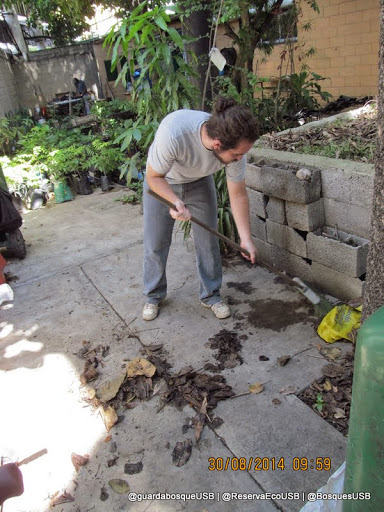
\includegraphics[scale=0.5]{imagenes/foto1}
    \caption{Barriendo en la Sociedad Amigos del Árbol. Luego estas hojas van al compostero.}
    \label{foto1}
\end{figure}

\item \textbf{Traslado de plantas:} la Sociedad de Amigos del Arbol donó alrededor de 200 árboles al vivero de la USB. Estos estaban destinados a ser plantados en la reserva ecológica USB con el fin de conmemorar aniversario 447 de de la ciudad de Caracas (jornada de plantación CCS 447). Por esta razón fue necesario movilizar estas plantas a la reserva ecológica de la USB.

\begin{figure}[H]
    \centering
    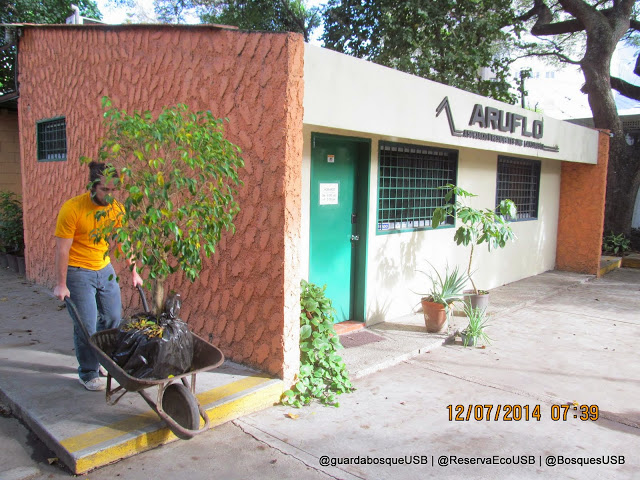
\includegraphics[scale=0.5]{imagenes/foto2}
    \caption{Trasladando las plantas de SADARBOL al camión que posteriormente las llevará a la reserva ecológica de la USB. Estos árboles se plantarán posteriormente en la jornada de arborización CCS 447.}
    \label{foto2}
\end{figure}

\end{itemize}

\subsection*{Mantenimiento del vivero forestal de la Universidad Simón Bolívar}
\addcontentsline{toc}{subsection}{Mantenimiento del vivero forestal de la Universidad Simón Bolívar}

\begin{itemize}

\item \textbf{Riego:} esta actividad consiste en proporcionar las cantidades adecuadas de agua todas las plantas que se encuentran en el vivero forestal. Esta actividad se realiza de manera periódica y es fundamental para el que las plantas crezcan rápido y en buenas condiciones.

\item \textbf{Elaboración de germinadores:} consiste en la siembra de una gran cantidad de semillas en guacales llenos de tierra. De esta forma se acelera el proceso de germinación, ya que es más sencillo sembrar varias semillas en un solo recipiente a sembrar una semilla por recipiente. Este proceso se lleva a cabo cuando se prevee que en determinado momento se debe repoblar el vivero. Las jornadas de plantación son la principal causa de la disminución de plantas en el vivero.

\item \textbf{Trasplante:} consiste en el traslado de una planta de un recipiente a otro. Es necesario realizar un trasplante cuando un recipiente se encuentra deteriorado o cuando la planta ha crecido lo suficiente y necesita de más tierra para seguir con su proceso de crecimiento. Este proceso se realiza muy frecuentemente cuando han germinado una gran cantidad de plantas anteriormente sembradas.

\begin{figure}[H]
    \centering
    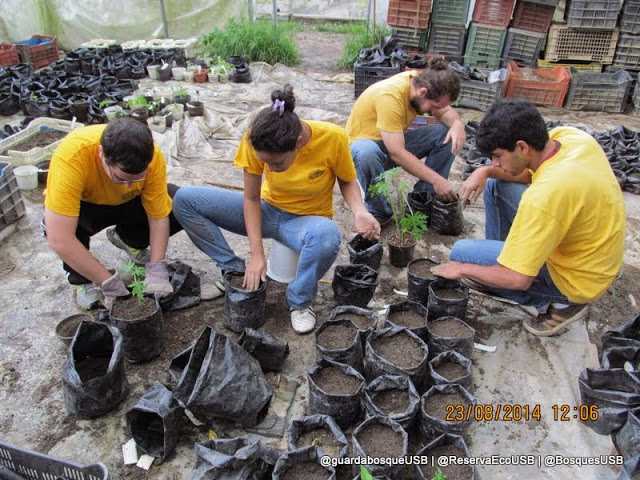
\includegraphics[scale=0.5]{imagenes/foto3}
    \caption{Trasplantando en el vivero forestal.}
    \label{foto3}
\end{figure}

\item \textbf{Cernido:} es el proceso de filtrado de la tierra. Esto se hace con el fin de eliminar piedras y desperdicios que en ella se puedan encontrar. De esta forma se obtiene una tierra de mejor calidad que luego es utilizada para realizar trasplantes y germinadores. El proceso de cernido se realiza recogiendo tierra con palas, la tierra se dispone en una malla metálica cilíndrica que luego se procede a girar y de esta forma (con la ayuda de la gravedad) se obtiene la tierra procesada. Es una actividad que se realiza periódicamente en el vivero.

\item \textbf{Organización:} consiste en clasificar y disponer las plantas que se encuentran en el vivero forestal según su tamaño y especie. Las plantas generalmente tienen que ser cargadas sin la ayuda de herramienta alguna (carretilla) y suele ser agotador ya que el vivero maneja cientos y hasta miles de plantas. Esta actividad se realiza constantemente.

\begin{figure}[H]
    \centering
    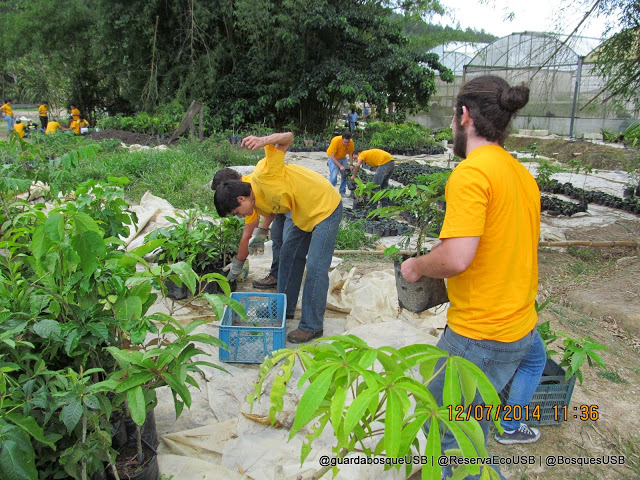
\includegraphics[scale=0.5]{imagenes/foto4}
    \caption{Clasificando y organizando plantas en el vivero forestal.}
    \label{foto4}
\end{figure}

\item \textbf{Desmalezamiento:} es el proceso de limpieza del terreno. Consiste en la eliminación de las plantas (que no son árboles) que compiten con los árboles por el terreno. Este proceso puede realizarse utilizando las manos en caso de que la maleza que está creciendo junto a las plantas en los recipientes en las que germinaron o fueron trasplantadas o con diversas con diversas herramientas si se está hablando de terreno al aire libre. Este proceso es se realizaba periódicamente en los recipientes donde se alojan las plantas y se realizaba en un terreno antes de realizar una jornada de arborización y eventualmente luego de la jornada.

\end{itemize}

\subsection*{Actividades en el campus universitario y en la reserva ecológica de la USB}
\addcontentsline{toc}{subsection}{Actividades en el campus universitario y en la reserva ecológica de la USB}

\begin{itemize}

\begin{figure}[h]
    \centering
    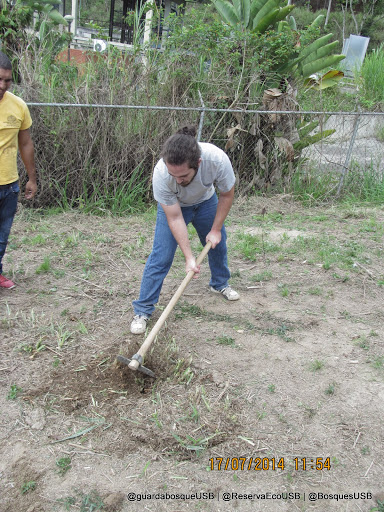
\includegraphics[scale=0.5]{imagenes/foto5}
    \caption{Desmalezando y preparando el terreno para la jornada de arborización Cargill de Venezuela.}
    \label{foto5}
\end{figure}


\item \textbf{``Ecorutas'':} es una actividad de concientización ambiental dirigida especialmente para niños y jóvenes. Se realiza un recorrido por el campus de la universidad conociendo los árboles emblemáticos de algunos estados del país que se encuentran en él. A lo largo del recorrido se realizan juegos educativos y se comparte información sobre los árboles y seres vivos que se encuentran en el campus. Concretamente se realizó la ``ecoruta'' con estudiantes de pregado de la USB, ellos formaban parte de un curso general dictado por Alicia Villamizar, profesora del Departamento de Estudios Ambientales de la USB. Esta actividad se realizó el 28 de octubre de 2014.

\begin{figure}[H]
    \centering
    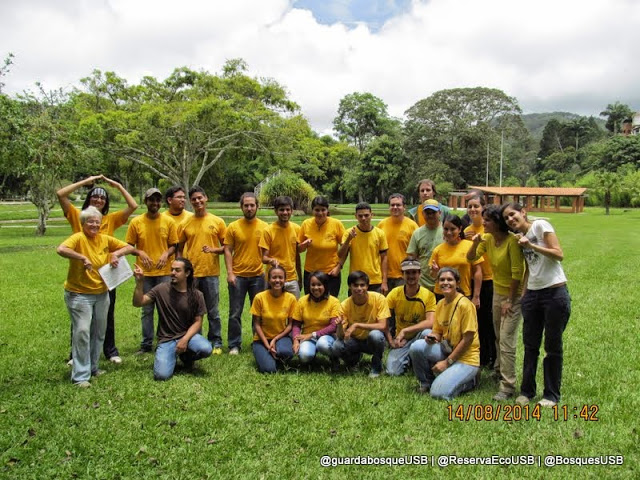
\includegraphics[scale=0.5]{imagenes/foto6}
    \caption{Preparación para ``ecorutas'' en el campus de la USB.}
    \label{foto6}
\end{figure}

\item \textbf{Jornada de reforestación con la empresa Cargill de Venezuela:} consistió en la coordinación y asistencia por parte de los guardabosques para que empleados de la empresa Cargill de Venezuela pudieran plantar alrededor de 300 árboles. Esta actividad se realizó en una parcela cercana al vivero forestal el día 19 de julio de 2014. También se aprovechó la oportunidad para resaltar la importancia y los beneficios que tiene la jornada. Luego de participar en la jornada de reforestación se realizaron juegos educativos para los niños.

\begin{figure}[H]
    \centering
    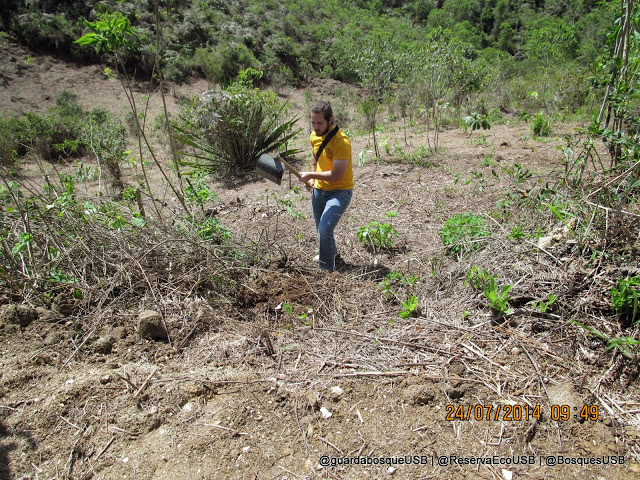
\includegraphics[scale=0.5]{imagenes/foto7}
    \caption{Haciendo escaleras para la jornada CCS 447.}
    \label{foto7}
\end{figure}

\item \textbf{Jornada de arborización Caracas 447:} la jornada se realizó en una parcela ubicada en la reserva ecológica de la USB (conocida como planta de gas). Fue una jornada donde participaron los habitantes de la Gran Caracas, en conmemoración a su aniversario 447. La jornada se efectuó el día 26 de julio de 2014 y se pretendía plantar 447 árboles pero debido al entusiasmo de las personas se terminó plantando más de 600 árboles. Los guardabosques plantaron y coordinaron a los miembros de la comunidad para poder realizar la jornada.

\begin{figure}[h]
    \centering
    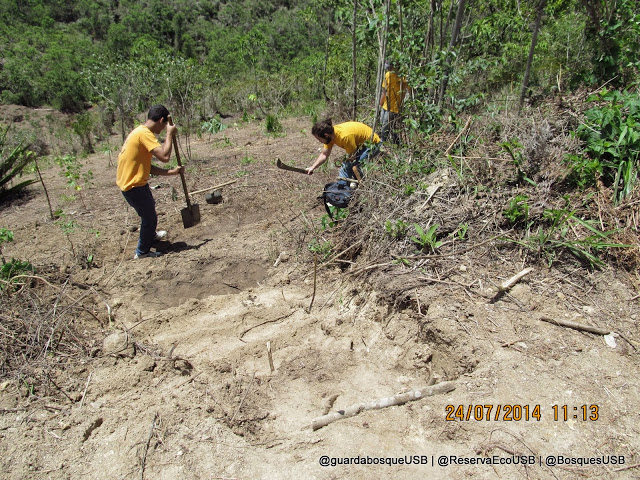
\includegraphics[scale=0.5]{imagenes/foto8}
    \caption{Terminando las escaleras para la jornada CCS 447.}
    \label{foto8}
\end{figure}

\begin{figure}[H]
    \centering
    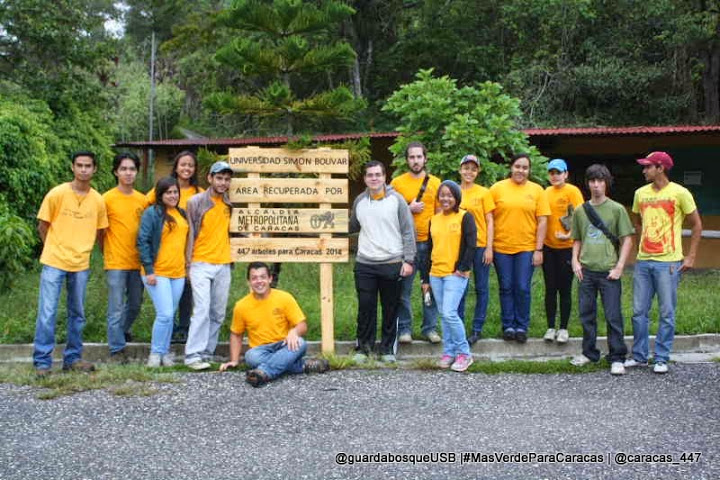
\includegraphics[scale=0.5]{imagenes/foto9}
    \caption{Iniciando el día de la jornada CCS 447.}
    \label{foto9}
\end{figure}

\begin{figure}[H]
    \centering
    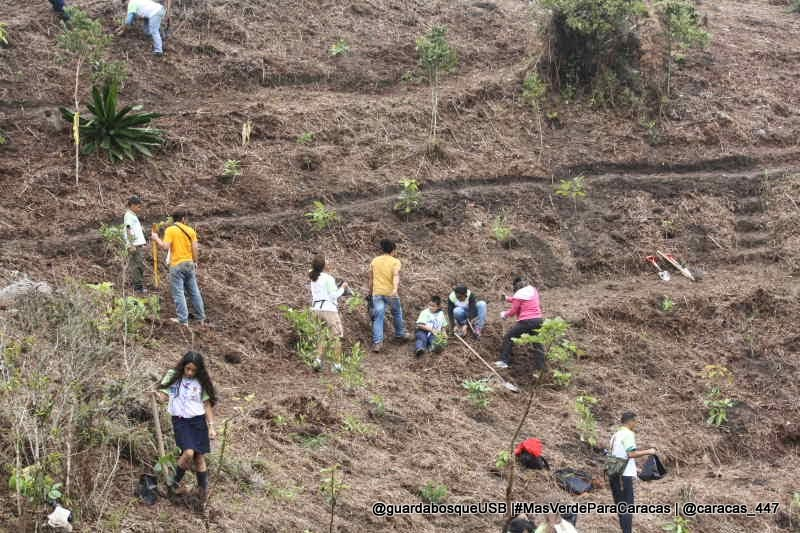
\includegraphics[scale=0.5]{imagenes/foto10}
    \caption{Plantando y orientando en la jornada CCS 447.}
    \label{foto10}
\end{figure}

\end{itemize}